\chapter{Split Ring Resonator}

In order to generate a plasma jet, a device known as a \textit{split ring resonator} (SSR) was used. An illustration of this device can be seen in figure \ref{fig:srr}. The design of a SSR is quite simple, consisting of a conducting ring, usually made of copper, laid on top of a dielectric substrate. The bottom of the dielectric consist of a ground plane that covers the entirety of the surface. This has the added benefit of dispersing the heat generated from the SSR. As seen in figure \ref{fig:srr}, there is a small gap made on the top surface that breaks the copper ring, which is where the plasma discharge occurs. 


\begin{figure}[h!]
	\centering
	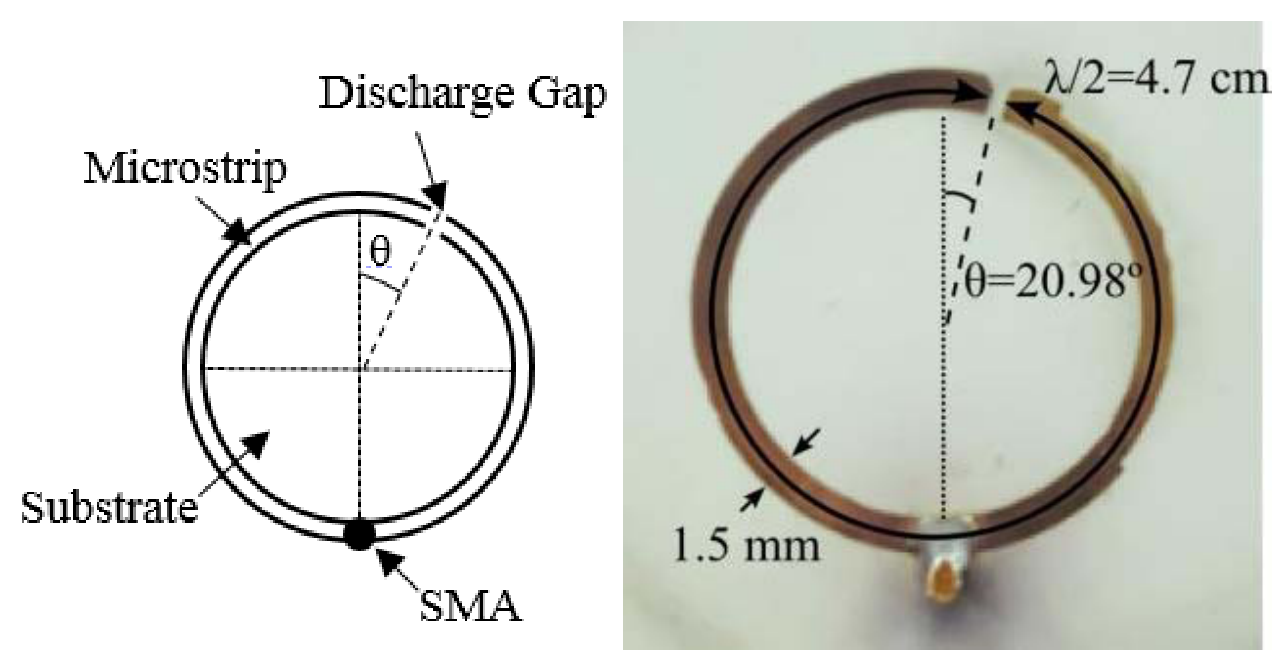
\includegraphics[width=0.7\linewidth]{chapter_4/figures/split_ring_resonator.png}
	\caption{Schematic (left) and photo (right) of SRR \cite{Dextre2017}.}
	\label{fig:srr}
\end{figure}

\section{Overview}

In order to achieve a discharge, an \textit{ultra high frequency} (UHF) voltage is applied to the SSR via the SMA connector. The exact frequency to be used is governed by two factors: the mean circumference (which is measured from the middle) of the top conducting ring and the dielectric constant of the substrate used. The mean circumference is usually designed to be half the wavelength corresponding to the desired frequency. The dielectric constant is required to determine the speed of light in the dielectric medium used. Thus, an equation for the frequency used for a given SSR is:

\begin{equation}
     f = \frac{c}{\lambda\sqrt{\varepsilon_r}}
     \label{eq:resonant_frequency}
\end{equation}

The reason why the mean circumference is designed to be half the desired wavelength is due to power efficiency. Due to this design, the ends of the SSR (i.e. where the gap is) will be $180 \circ$ out of phase from each other. Because of this, when one end of the SRR is at the peak of the AC cycle, the other will be at a trough; thus the potential difference between the two ends has been doubled. This geometric trick allows for the doubling of the strength of the electric field at a constant power. 

Astute readers may notice another peculiarity with the SSR seen in figure \ref{fig:srr}, in that it is not symmetrical. Instead, the discharge gap appears to be offset towards one side of the device. This is deliberate as the offset gap allows for the impedance matching of the SRR to the impedance of the power supply used, thus maximising the power transfer. This offset angle is measured from the very centre of the ring, and is determined using the expression:

\begin{equation}
	\theta = arccos(1 - \frac{Z_{in} \pi}{Z_0 Q})
	\label{eq:offset_angle}
\end{equation}


where $Z_{in}$ is the input impedance of the power supply, $Q$ is the quality factor, and $Z_0$ is the characteristic impedance of the SRR. Typically, the input impedance of many power supplies is 50 $\Omega$. The characteristic impedance can be determined by the width of the top copper trace, the thickness of the dielectric substrate, and the dielectric constant of the substrate. As for the quality factor, this parameter is given on the data sheet of the substrate used.

\section{Production}

The SSR device needed for this project requires a slight modification to the design compared to the traditional SSR. In order to create a small jet of plasma, through holes are needed at the region of the gap of the SSR. This would allow the gases to react with the plasma, then pass through the hole.

However, to determine if this small change had any significant effects on the behaviour of the SSR, simulations were run to better understand what was going on. Specifically, \textit{Particle-in-cell} (PIC) simulations were used; and the software used is called \textit{XOOPIC}. Further information on PIC simulations and XOOPIC can be found in the appendices. 

\subsection{Simulations}

Multiple different simulations were run to understand the characteristics of the plasma, however they could be broadly broken down into three groups. For all these simulations, a cross sectional plane of the discharge gap of the SSR was modelled. The reasoning for this was that the plasma formed would typically be constrained around the gap. Though the ring of the SRR is a circle, the discharge gap is small relative to the overall device, hence can be approximated to be a rectangle. Thus such a simulation would be valid assuming that the electric field across the gap is constant along all points of the ring. For all the following simulations, the parameters can be found in table \ref{tb:basic_simulation_parameters} unless specified otherwise.

\begin{table}[h!]
	\caption{Simulation parameters of SSR in XOOPIC.}
	\vspace{3 pt}
	\centering
	\begin{tabular}{l r l}
		Parameters               & Value    & Units  \\
		\hline 
		Domain x-axis            & 1.0      & mm     \\
		Domain y-axis            & 2.5  	& mm     \\
		Dielectric thickness     & 500      & $\mu$m \\
		Dielectric constant      & 3.66     &        \\
		Equipotential thickness  & 40       & $\mu$m \\
		Gas pressure             & 780      & Torr   \\
		Gas temperature          & 25       & meV    \\
		Potential Difference     & 150      & V      \\
		Frequency                & 1        & GHz    \\
		Time step                & 0.1      & ps
	\end{tabular}
	\label{tb:basic_simulation_parameters}
\end{table}

The first of these simulation groups was to simply study the effects of introducing a through hole to the SSR. For this test, all simulation parameters were kept identical, the only difference would be the introduction design of the gap. An visualisation of the simulations could be seen in the figure below. In figure \ref{fig:SSR_no_gap_start}, the dielectric substrate (seen in gold) and the bottom electrode (seen in green) is kept intact as a single structure, whereas the top electrode (seen in yellow) is split. However in \ref{fig:SSR_hole_comparison_start}, all three layers of the SSR are split into two. The size of the discharge gap chosen was 240 $\mu$m, the dielectric constant of the substrate was 3.66, and the voltage used was 150 V at 1 GHz. 

\begin{figure}
\centering
\begin{subfigure}{0.5\textwidth}
  \centering
  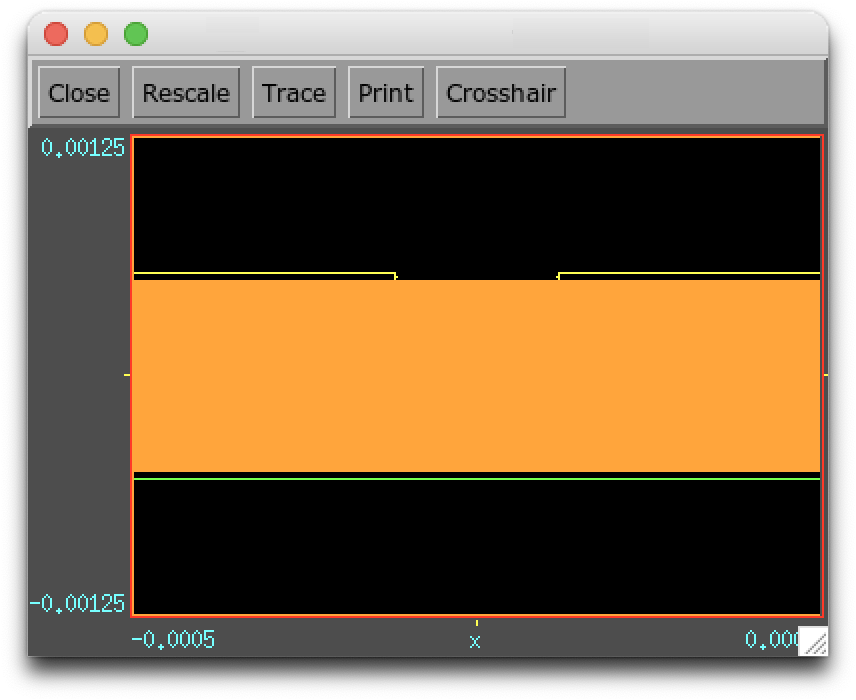
\includegraphics[width=0.9\linewidth]{chapter_4/figures/SSR_no_gap_start.png}
  \caption{Cross section of SSR without hole in gap.}
  \label{fig:SSR_no_gap_start}
\end{subfigure}%
\begin{subfigure}{.5\textwidth}
  \centering
  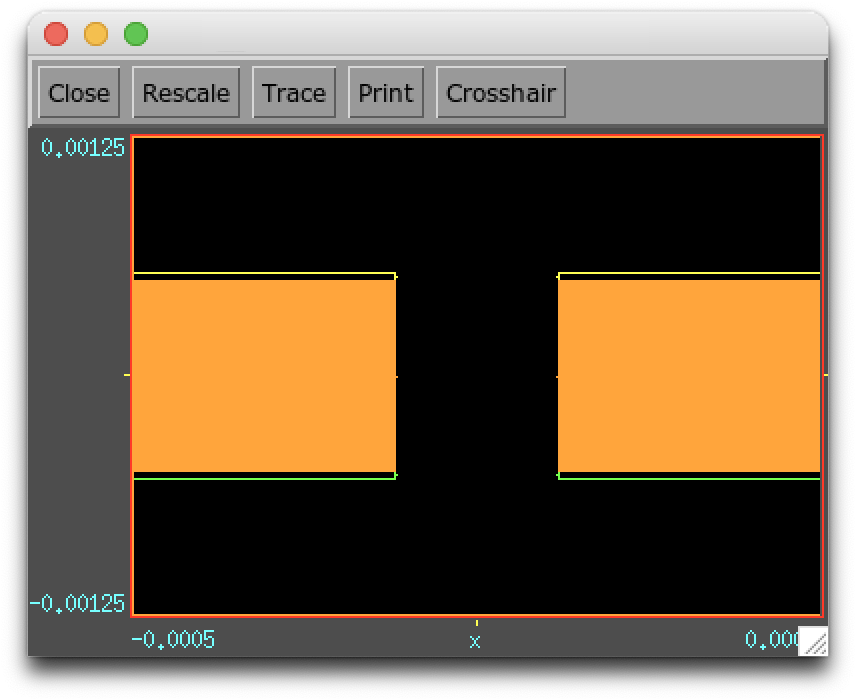
\includegraphics[width=0.9\linewidth]{chapter_4/figures/SSR_with_gap_start.png}
  \caption{Cross section of SSR with hole in gap.}
  \label{fig:SSR_with_gap_start}
\end{subfigure}
\caption{A comparison of SSR with and without hole in gap.}
\label{fig:SSR_hole_comparison_start}
\end{figure}

The results of the simulation after it stabilised can be seen in figure \ref{fig:SSR_hole_comparison_stabilise}. The immediate difference that can be observed is the fact that the ions and electrons, represented as blue and orange dots respectively, tended to `sit' deeper into the gap in the case with the through hole. Intuitively, this would make sense as these particles are not colliding with the substrate (which in XOOPIC meant that they were removed from the simulation domain). Additionally, it was hypothesised that strength of the electric field between the top electrodes and the ground plane could potentially play an effect in how deep the ions and electrons `sit' in the gap of the SSR.

\begin{figure*}
    \centering
    \begin{subfigure}[b]{0.475\textwidth}
        \centering
        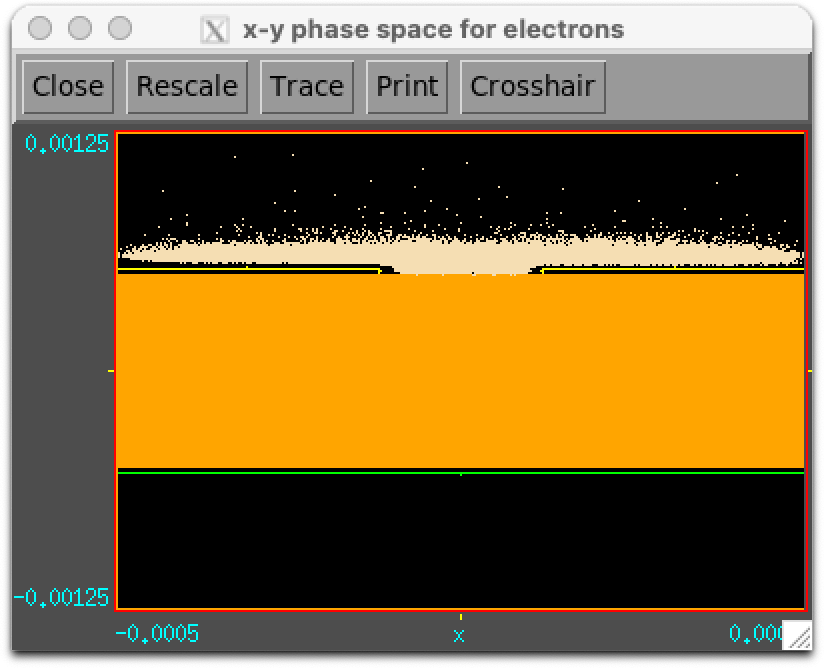
\includegraphics[width=\textwidth]{chapter_4/figures/SSR_no_hole_electrons.png}
        \caption[]%
        {{\small Plot of electrons in SSR without hole in gap.}}    
        \label{fig:SSR_no_hole_electrons}
    \end{subfigure}
    \hfill
    \begin{subfigure}[b]{0.475\textwidth}  
        \centering 
        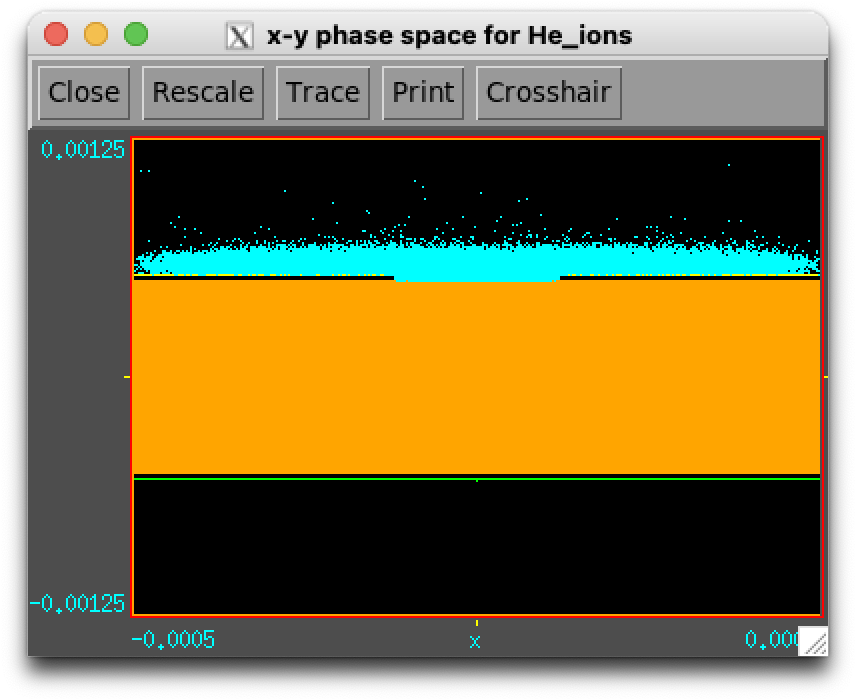
\includegraphics[width=\textwidth]{chapter_4/figures/SSR_no_hole_ions.png}
        \caption[]%
        {{\small  Plot of ions in SSR without hole in gap.}}    
        \label{fig:SSR_no_hole_ions}
    \end{subfigure}
    \vskip\baselineskip
    \begin{subfigure}[b]{0.475\textwidth}   
        \centering 
        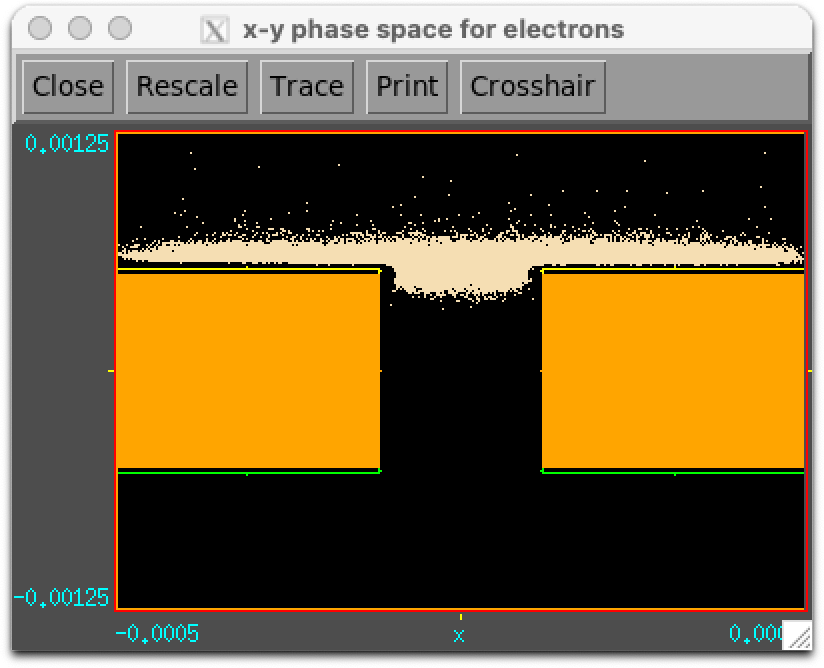
\includegraphics[width=\textwidth]{chapter_4/figures/SSR_with_hole_electrons.png}
        \caption[]%
        {{\small Plot of electrons in SSR with hole in gap.}}    
        \label{fig:SSR_with_hole_electrons}
    \end{subfigure}
    \hfill
    \begin{subfigure}[b]{0.475\textwidth}   
        \centering 
        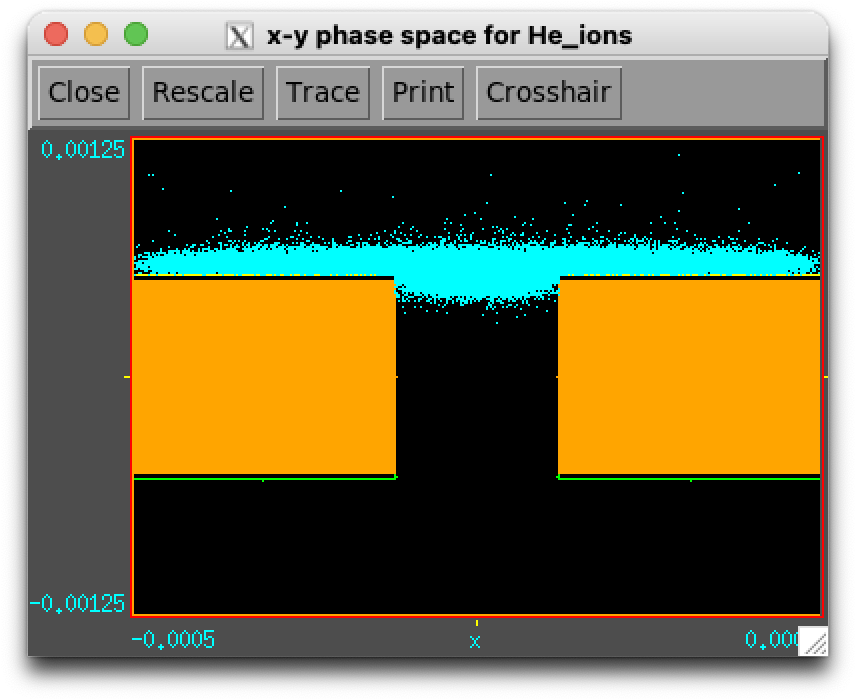
\includegraphics[width=\textwidth]{chapter_4/figures/SSR_with_hole_ions.png}
        \caption[]%
        {{\small Plot of ions in SSR with hole in gap.}}    
        \label{fig:SSR_with_hole_ions}
    \end{subfigure}
    \caption[]
    {\small Comparison of SSR with and without hole in gap.} 
    \label{fig:SSR_hole_comparison_stabilise}
\end{figure*}

This leads into the second group of simulations that were run, where the separation distance between the top and bottom electrodes were investigated, which also had the added benefit of identifying if the ideal dielectric substrate thickness to be used when manufacturing the SSR. The parameters used for the size of the gap, the dielectric constant of the substrate, and the potential difference were kept the same as the first group. As for the dielectric thickness, simulations were run with values of 0.2 mm, 0.5 mm, 1.0 mm, 1.5 mm, and 2.0 mm. 

From the cross sectional view of the density plot of electrons in figure \ref{fig:SSR_dielectric_comparison_stabilise}, all simulations performed quite similarly. The electrons seem to extend through the gap by roughly the same distance. However, even though the dielectric thickness did not play a large role in the plasma, it would be preferable to choose a thicker dielectric for the sturdiness of the board. 

The final group of simulations run were to establish the effect of the discharge gap widths. The sizes used were a gap width of 120 $\mu$m, 240 $\mu$m, 360 $\mu$m, and 480 $\mu$m. 

\begin{figure}[h!]
	\centering
	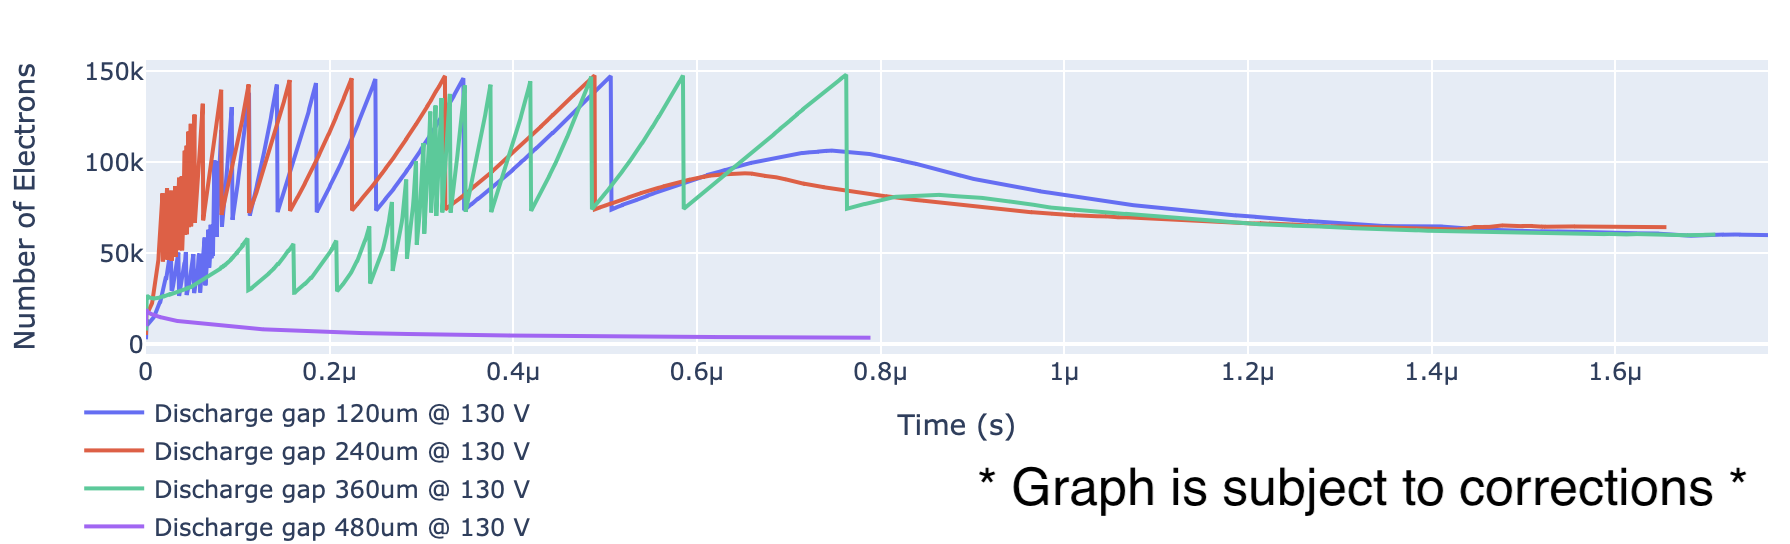
\includegraphics[width=\linewidth]{chapter_4/figures/num_elec_gap.png}
	\caption{Time series plot of number of electrons across different discharge gaps.}
	\label{fig:num_elec_gap}
\end{figure}

The results of these simulations can be seen in figure \ref{fig:num_elec_gap}. From these tests, only three simulations were successful as the run with a gap width of 480 $\mu$m lost all the seed electrons. The most likely explanation for this behaviour was that the voltage used (150 V) was not sufficient to ignite a discharge. As for the other three runs, the big difference seemed to be the initial growth rate. A gap width of 240 $\mu$m appeared to be the optimum. One would expect that the smallest gap width would perform the best, however as seen by Paschen's law (refer to Chapter \ref{sec:paschens_law}), reducing the distance between electrodes too much would cause the electrons to be simply lost to the electrode. This could possibly explain why the run with a gap width of 120 $\mu$m underperformed.

\begin{figure*}
    \centering
    \begin{subfigure}[b]{0.475\textwidth}
        \centering
        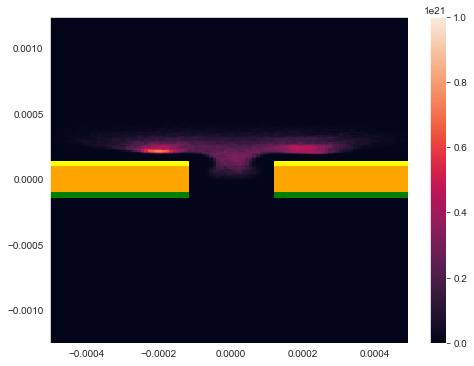
\includegraphics[width=\textwidth]{chapter_4/figures/SSR_dielectric_1.png}
        \caption[]%
        {{\small Dielectric thickness of 0.2 mm.}}    
        \label{fig:SSR_dielectric_0.2mm}
    \end{subfigure}
    \hfill
    \begin{subfigure}[b]{0.475\textwidth}  
        \centering 
        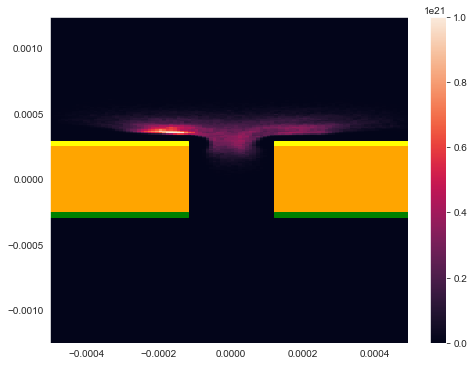
\includegraphics[width=\textwidth]{chapter_4/figures/SSR_dielectric_2.png}
        \caption[]%
        {{\small  Dielectric thickness of 0.5 mm.}}    
        \label{fig:SSR_dielectric_0.5mm}
    \end{subfigure}
    \vskip\baselineskip
    \begin{subfigure}[b]{0.475\textwidth}   
        \centering 
        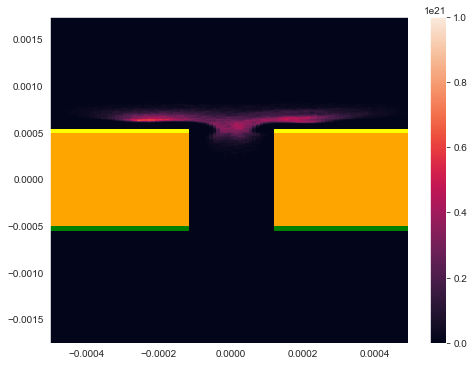
\includegraphics[width=\textwidth]{chapter_4/figures/SSR_dielectric_3.png}
        \caption[]%
        {{\small Dielectric thickness of 1.0 mm.}}    
        \label{fig:SSR_dielectric_1.0mm}
    \end{subfigure}
    \hfill
    \begin{subfigure}[b]{0.475\textwidth}   
        \centering 
        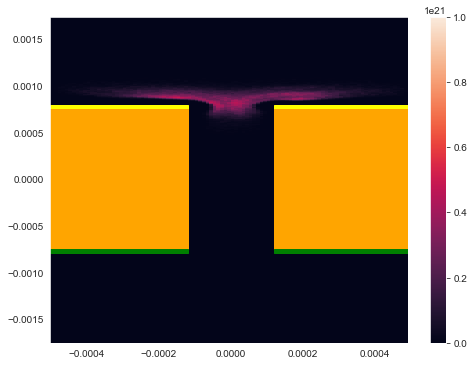
\includegraphics[width=\textwidth]{chapter_4/figures/SSR_dielectric_4.png}
        \caption[]%
        {{\small Dielectric thickness of 1.5 mm.}}    
        \label{fig:SSR_dielectric_1.5mm}
    \end{subfigure}
    \vskip\baselineskip
    \begin{subfigure}[b]{0.475\textwidth}   
        \centering 
        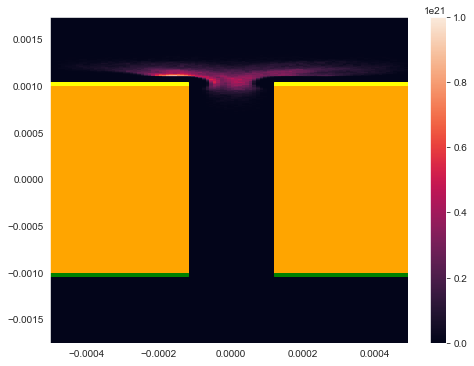
\includegraphics[width=\textwidth]{chapter_4/figures/SSR_dielectric_5.png}
        \caption[]%
        {{\small Dielectric thickness of 2.0 mm.}}    
        \label{fig:SSR_dielectric_2.0mm}
    \end{subfigure}
    \caption[]
    {\small Comparison of dielectric thickness on SSR with hole in gap.} 
    \label{fig:SSR_dielectric_comparison_stabilise}
\end{figure*}

\subsection{Design}

Armed with this information, a design of the SSR to be used was made. The first step was to select the PCB substrate to be used, as its dielectric constant is a central parameter for all other calculations of the SSR. The material selected was the RO4350B\textsuperscript{TM} material from Rogers corporation. This specific material was chosen as it is designed for high power UHF designs, and its relatively low fabrication costs. Additionally, the RO4350B\textsuperscript{TM} material did not require any special treatments or procedures to produce a through hole. According to its data sheet, the RO4350B\textsuperscript{TM} board has a dielectric constant of 3.66, and a dissipation factor of 0.0031 (which can be converted to the quality factor).  

The next step was to determine the resonant frequency for the SSR. Ideally, a higher resonant frequency would improve the quality factor, reducing power losses and making it more likely that a plasma discharge occurs. However, a frequency that was too high would increase power requirements and would also reduce the size of the SSR. Therefore, a compromise between the two needed to be struck, and a target frequency 950 MHz was chosen. 

Feeding this number into equation \ref{eq:resonant_frequency}, the corresponding wavelength was 0.165 m. Since the circumference of the SSR is given as $\lambda/2$, this meant that the design had a circumference of 8.25 cm; which was a radius of approximately 1.3 cm. 

The next step was to determine the characteristic impedance. Conventionally, this impedance should be close to the value of the input impedance, which for power supply used was 50 $\Omega$. As mentioned earlier in this chapter, three factors dictate the value of this parameter. The dielectric constant of the substrate was 3.66, a fixed value based on the material used. As stated in the previous section, a thicker dielectric substate would be preferable. The RO4350B\textsuperscript{TM} material came in a thickness of 0.5 mm, 0.8 mm, and 1.55 mm; with the costs increasing with thickness. Thus, as compromise between the structural rigidity PCB and cost, a thickness of 0.8 mm was selected. By using the equations by Wheeler in \cite{wheeler_1977}, a trace width of approximately 1.7 mm would produce a characteristic impedance of 50.1 $\Omega$.

Finally using equation \ref{eq:offset_angle}, the offset angle of the SSR was calculated. As from the datasheet, the dissipation factor of the RO4350B\textsuperscript{TM} material is 0.0031. The reciprocal of this value was taken to determine the quality factor, which was 323. This would give a gap with an offset angle of 7.99. Again based on the simulations above, the ideal gap width was 240 $\mu$m, however the minimum size drill hole size would limiting factor when manufacturing, hence the gap width was slightly increased to 250 $\mu$m.

With these parameters known, the next stage was to create the PCB design. This was done using the open-sourced PCB design software called \textit{KiCad}. An illustration of the final design can be seen in figure \ref{fig:srr_cad}. As seen from the figure, four SSR designs were made. These were done to test various gap designs that could not be replicated using XOOPIC simulations. These designs could be broken down into two categories: single versus multiple drill hole in SSR gap; and the presence versus absence of `finger-like' copper pours next to the SSR gap. The permutations of these categories resulted in the four designs, with a close up image of each seen in figure \ref{fig:ssr_cad_close_up}. All four designs also used an SMA connector as the input source. 

\begin{figure}[h!]
	\centering
	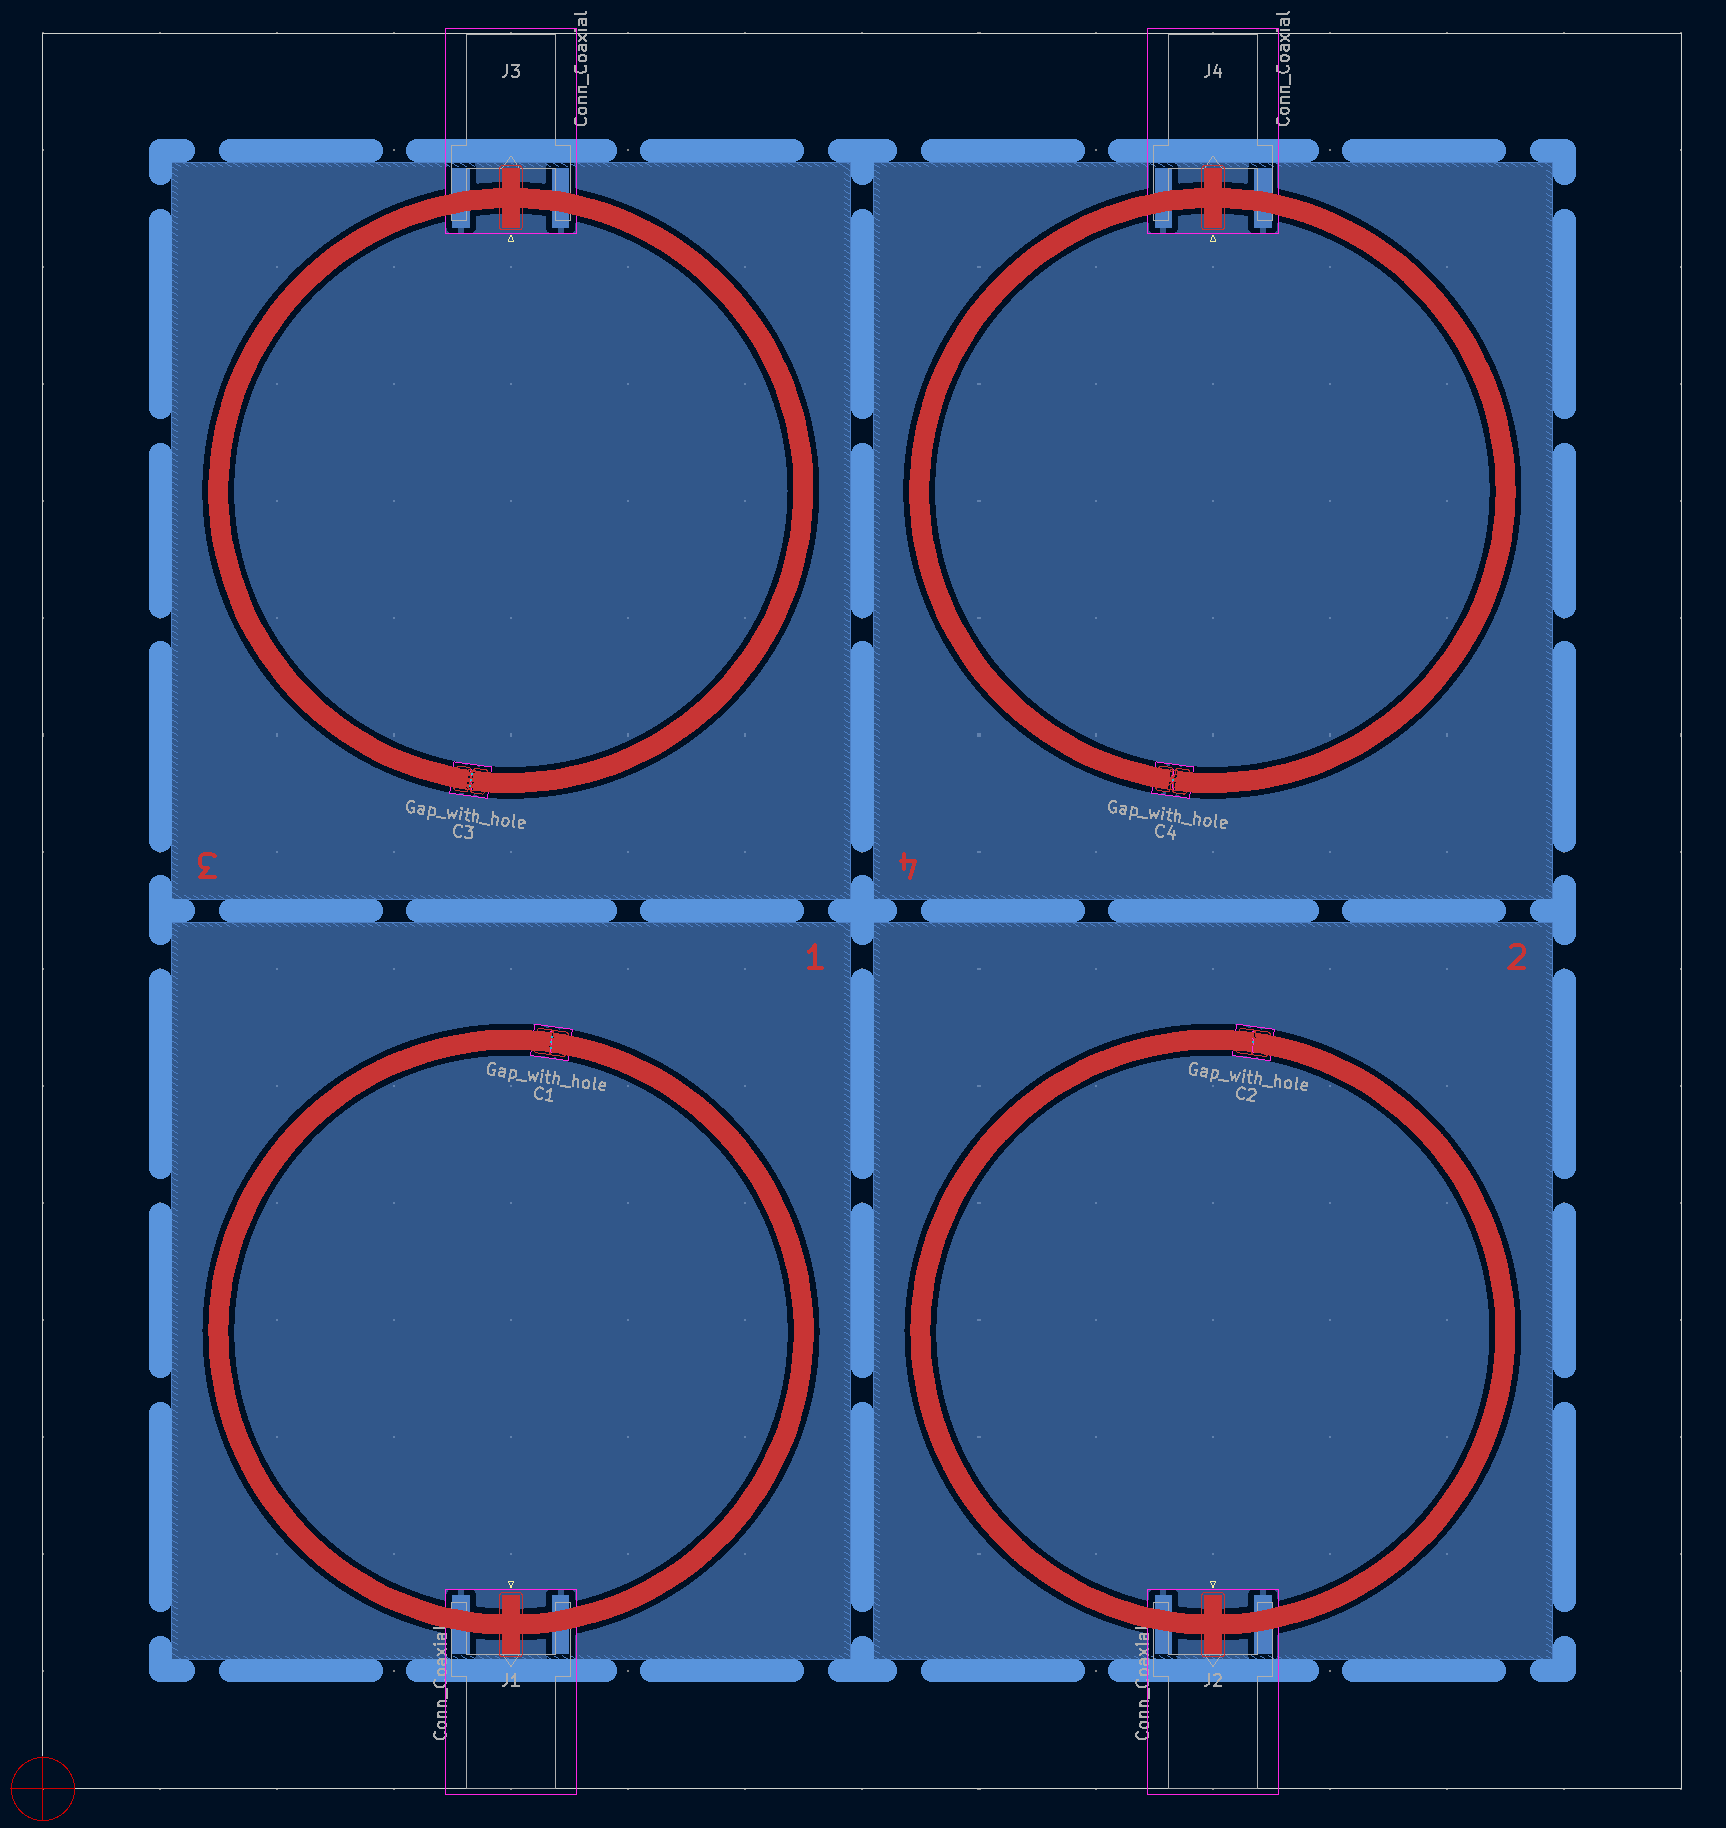
\includegraphics[width=0.9\linewidth]{chapter_4/figures/SSR_CAD.png}
	\caption{PCB design of SSR in KiCad.}
	\label{fig:srr_cad}
\end{figure}

\begin{figure*}
    \centering
    \begin{subfigure}[b]{0.475\textwidth}
        \centering
        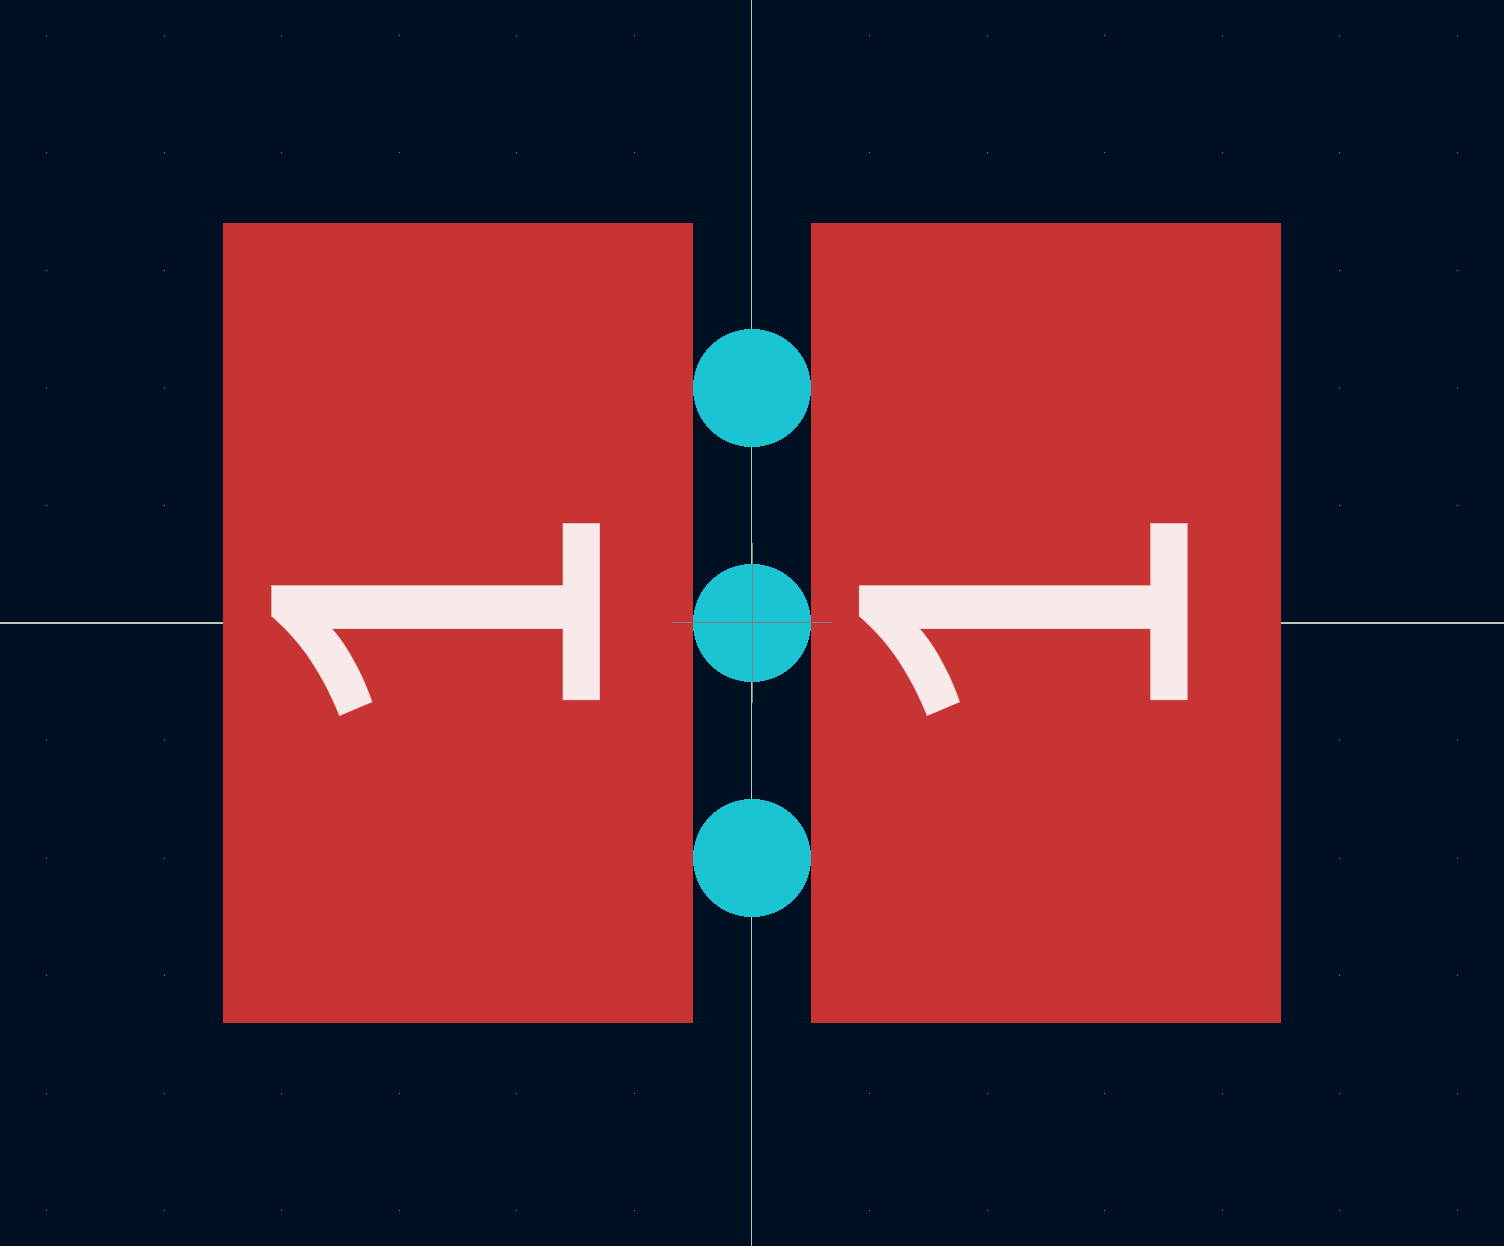
\includegraphics[width=\textwidth]{chapter_4/figures/SSR_CAD_hole_1.png}
        \caption[]%
        {{\small Design 1 - Multiple holes, no `fingers'.}}    
        \label{fig:design_1}
    \end{subfigure}
    \hfill
    \begin{subfigure}[b]{0.475\textwidth}  
        \centering 
        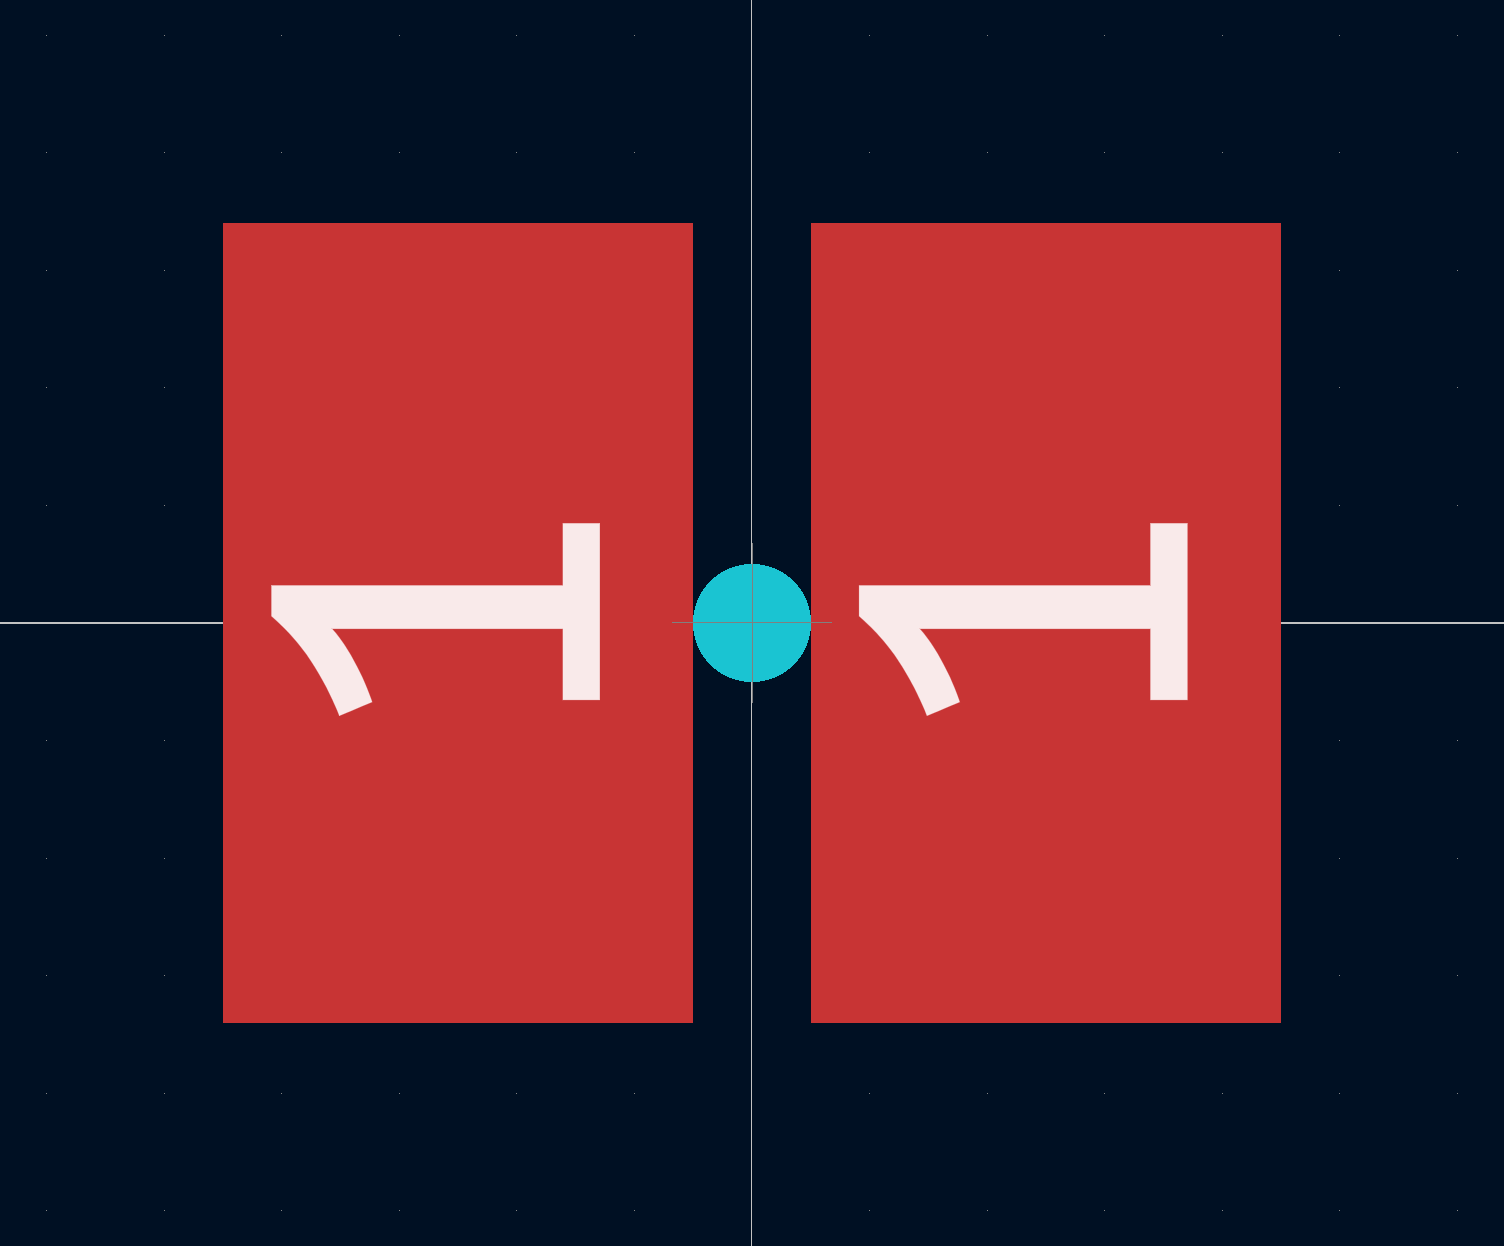
\includegraphics[width=\textwidth]{chapter_4/figures/SSR_CAD_hole_2.png}
        \caption[]%
        {{\small  Design 2 - Single hole, no `fingers'.}}    
        \label{fig:design_2}
    \end{subfigure}
    \vskip\baselineskip
    \begin{subfigure}[b]{0.475\textwidth}   
        \centering 
        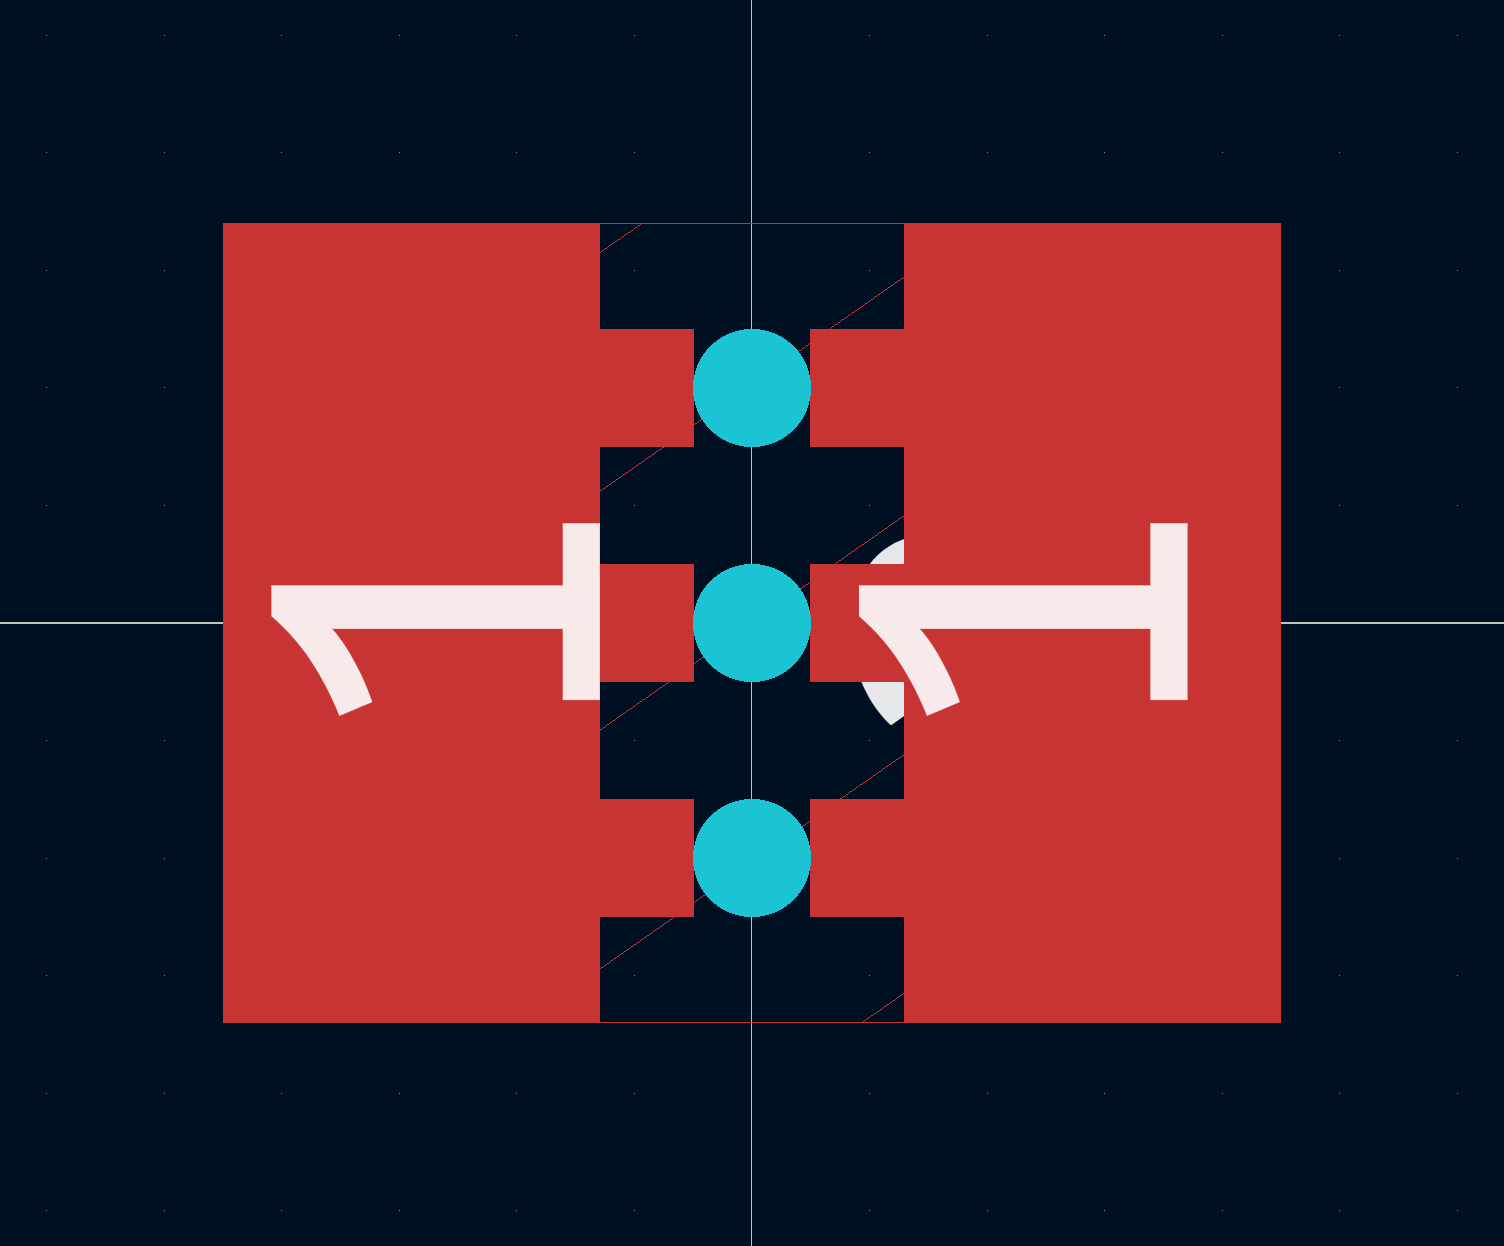
\includegraphics[width=\textwidth]{chapter_4/figures/SSR_CAD_hole_3.png}
        \caption[]%
        {{\small Design 3 - Multiple holes, with `fingers'.}}    
        \label{fig:design_3}
    \end{subfigure}
    \hfill
    \begin{subfigure}[b]{0.475\textwidth}   
        \centering 
        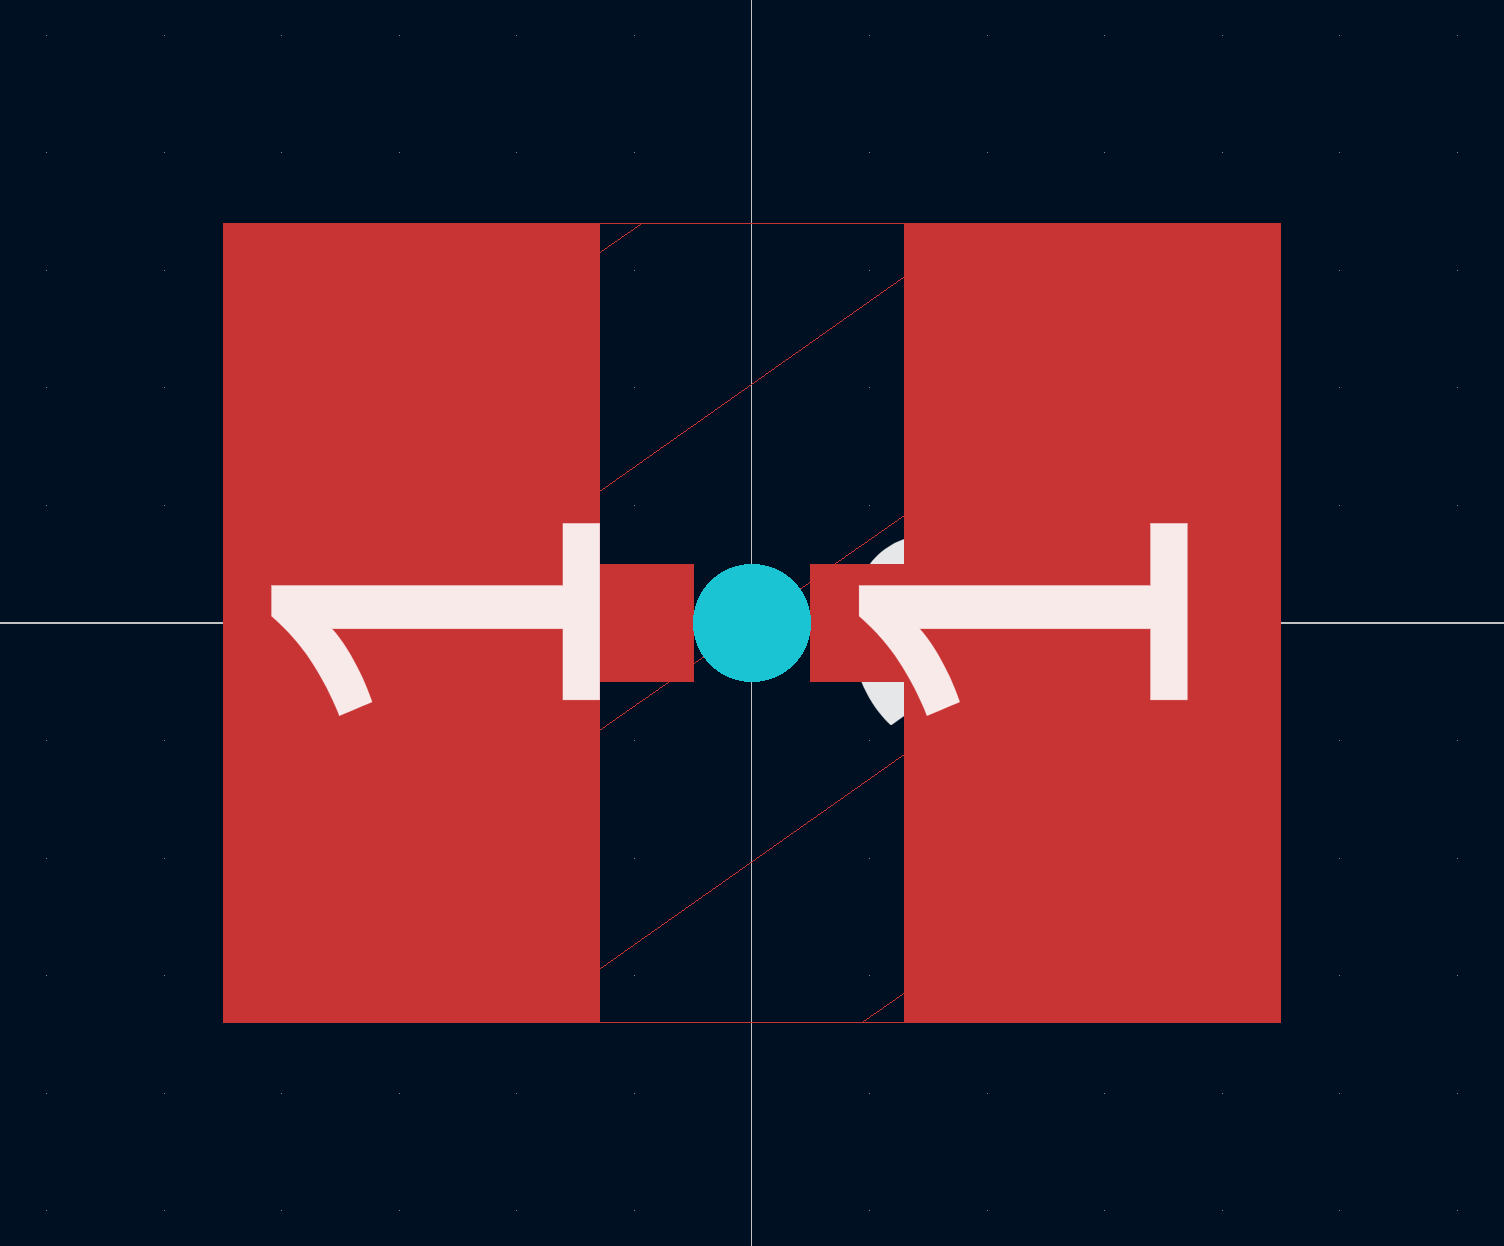
\includegraphics[width=\textwidth]{chapter_4/figures/SSR_CAD_hole_4.png}
        \caption[]%
        {{\small Design 4 - Single hole, with `fingers'.}}    
        \label{fig:design_4}
    \end{subfigure}
    \caption[]
    {\small Close up of SSR gap designs.} 
    \label{fig:ssr_cad_close_up}
\end{figure*}

\section{Testing}




